\documentclass[11pt, a4paper, leqno]{article}
\usepackage{a4wide}
\usepackage[T1]{fontenc}
\usepackage[utf8]{inputenc}
\usepackage{float, afterpage, rotating, graphicx}
\usepackage{epstopdf}
\usepackage{longtable, booktabs, tabularx}
\usepackage{fancyvrb, moreverb, relsize}
\usepackage{eurosym, calc}
% \usepackage{chngcntr}
\usepackage{amsmath, amssymb, amsfonts, amsthm, bm}
\usepackage{caption}
\usepackage{mdwlist}
\usepackage{xfrac}
\usepackage{setspace}
\usepackage{xcolor}
\usepackage{subcaption}
\usepackage{minibox}
% \usepackage{pdf14} % Enable for Manuscriptcentral -- can't handle pdf 1.5
% \usepackage{endfloat} % Enable to move tables / figures to the end. Useful for some submissions.



\usepackage{natbib}
\bibliographystyle{rusnat}




\usepackage[unicode=true]{hyperref}
\hypersetup{
    colorlinks=true,
    linkcolor=black,
    anchorcolor=black,
    citecolor=black,
    filecolor=black,
    menucolor=black,
    runcolor=black,
    urlcolor=black
}


\widowpenalty=10000
\clubpenalty=10000

\setlength{\parskip}{1ex}
\setlength{\parindent}{0ex}
\setstretch{1.5}


\begin{document}

\title{Final Projecct: Rossmann Sales Prediction \thanks{Aiwei Huang, Universität Bonn. Email: \href{mailto:aimeewong1988@gmail.com}{\nolinkurl{aimeewong1988 [at] gmail [dot] com}}.}}

\author{Aiwei Huang}

\date{
{\bf Preliminary -- please do not quote}
\\[1ex] 
\today
}

\maketitle


%\begin{abstract}
%	Some abstract here.
%\end{abstract}
\clearpage

\section{Introduction} % (fold)
Rossmann is Germany's second-largest drug store chain which operates over 3,790 stores in 7 European countries. Historical data including sales were given by Rossmann in order to forecast daily sales six weeks in advance. Apparently, different factors associated with distinguishable regression models results in various accuracy in sales prediction. In the later sections, starting with correlation analysis between sales and distinct factors, after important features being extracted from raw data, 6 different algorithms are employed to this problem: linear regression, ridge regression, lasso regression, decision tree, random forest, gradient boosting and mean squared error (MSE) is applied as predictive veracity assessment.

% section introduction (end)
\section{Data Description and Preprocessing}


\subsection{Datasets and Features}

All data used in the project is provided by Kaggle. Historical data including sales is represented in train dataset which contains 1,017,209 samples and 9 features of marketing information are embodied in each sample. Store dataset consists of 1,115 samples with each representing 10 features of supplemental information about the stores. Test dataset embraces all stores that are still open and date interval of 6 weeks.

Although most of the data fields are self-explanatory, the following ones still need to be disclosed since they lay the groundwork for the data visualization.

\begin{itemize}

    \item \textit{ID} -- an Id that represents a (Store, Date) duple within the test set
    \item \textit{Store} -- a unique Id for each store
    \item \textit{Open} -- an indicator for whether the store was open: 0 = closed, 1 = open
    \item \textit{StateHoliday} -- indicates a state holiday. Normally all stores, with few exceptions, are closed on state holidays. Note that all schools are closed on public holidays and weekends. a = public holiday, b = Easter holiday, c = Christmas, 0 = None
    \item \textit{SchoolHoliday} -- indicates if the (Store, Date) was affected by the closure of public schools
    \item \textit{StoreType} -- differentiates between 4 different store models: a, b, c, d
    \item \textit{Assortment} -- describes an assortment level: a = basic, b = extra, c = extended
    \item \textit{Promo} -- indicates whether a store is running a promo on that day
    \item \textit{Promo2} -- Promo2 is a continuing and consecutive promotion for some stores: 0 = store is not participating, 1 = store is participating
    \item \textit{PromoInterval} -- describes the consecutive intervals Promo2 is started, naming the months the promotion is started anew

\end{itemize}

\subsection{Data Visualization}

After joining train dataset with additional store supplemental information by merging store dataset into train dataset and then replace null data, I am able to look deep into the data via data visualization.

As shown in Fig \ref{fig:Correlation}, the correlations visualised with the help of heatmap. Features like 'Customers', 'Open', 'Promo' have certain positive correlation with 'Sales' and the correlation between 'Sales' and 'DayOfWeek' is negative. Heatmap also provide a strong evidence for choosing important features in the later section.
\begin{figure}[ht]
\centering
\includegraphics[width=0.7\columnwidth]{../../out/figures/train_store_coorr.pdf}
\caption{Correlation coefficients are calculated based on train and store dataset.}
\label{fig:Correlation}
\end{figure}

Calculating the mean of monthly sales of each store, Fig \ref{fig:Monthly_Sales} reveals a time series of average Sales for each store. Seasonal sales explosions can be obviously observed at the end of year 2013 and 2014. Therefore, 2 mechanisms could be adopted to achieve the goal: additive mechanism using linear-scale and relative change mechanisum for which log-scale is critical\cite{euser2008practical,newman1993regression}.

\begin{figure}[ht]
\centering
\includegraphics[width=0.7\columnwidth]{../../out/figures/monthly_sales.pdf}
\caption{Time Series of monthly Sales.}
\label{fig:Monthly_Sales}
\end{figure}

Fig \ref{fig:Daily_} displays average store sales corresponding to each weekday. It is interesting to note that day 7 have the largest amount of sales among all the weekdays in each year. Only a few stores opened in day 7 but they share the largest average sales.
\begin{figure}[ht]
\centering
\includegraphics[width=0.9\columnwidth]{../../out/figures/dayofweeksales.pdf}
\caption{Daily average Store Sales.}
\label{fig:Daily_}
\end{figure}

The relations between sales and store type/ assortment shown as Fig \ref{fig:StoreType_}. Compares with StoreType a,c,d, sales of StoreType b stands out. Assortment b contributes more sales than the other and their influences on sales have some regular pattern.
\begin{figure}[ht]
\centering
\includegraphics[width=0.8\columnwidth]{../../out/figures/storetype_assortment_sales.pdf}
\caption{StoreType and Assortment impact Sales.}
\label{fig:StoreType_}
\end{figure}

\section{Feature Selection and Data Cleaning}
Feature number growth would not only rise the risk of overfitting, but also increase model training time, therefore, feature selection is an absolutely crucial step for model construction\cite{kira1992practical,guyon2003introduction}. Feature importance is an inbuilt class that comes with Tree Based Classifiers.
I would like to use this method combine with Heatmap in data visualization to select features.
First have a look at Figure 1, 'Promo2SinceYear' and 'Promo2' are too strong related, only one of them should be left, so I would drop 'Promo2SinceYear' in data cleaning. The correlation coefficient of pair 'Sales' and 'CompetitionOpenSinceYear' is too low, which means there is almost none relationshiop between them. Hence, 'CompetitionOpenSinceYear' should be excluded.

In order to bring more data into feature selection, I convert categorical variables such as 'StoreType','Assortment' into indicator variables. Sklearn provides a great tool: random forest algorithm for feature importance measurement \cite{liaw2002classification} by looking at how much the tree nodes, which use that feature, reduce impurity across all trees in the forest. to show importance of features as Fig \ref{fig:Importance Of Features}.
\begin{figure}[ht]
\centering
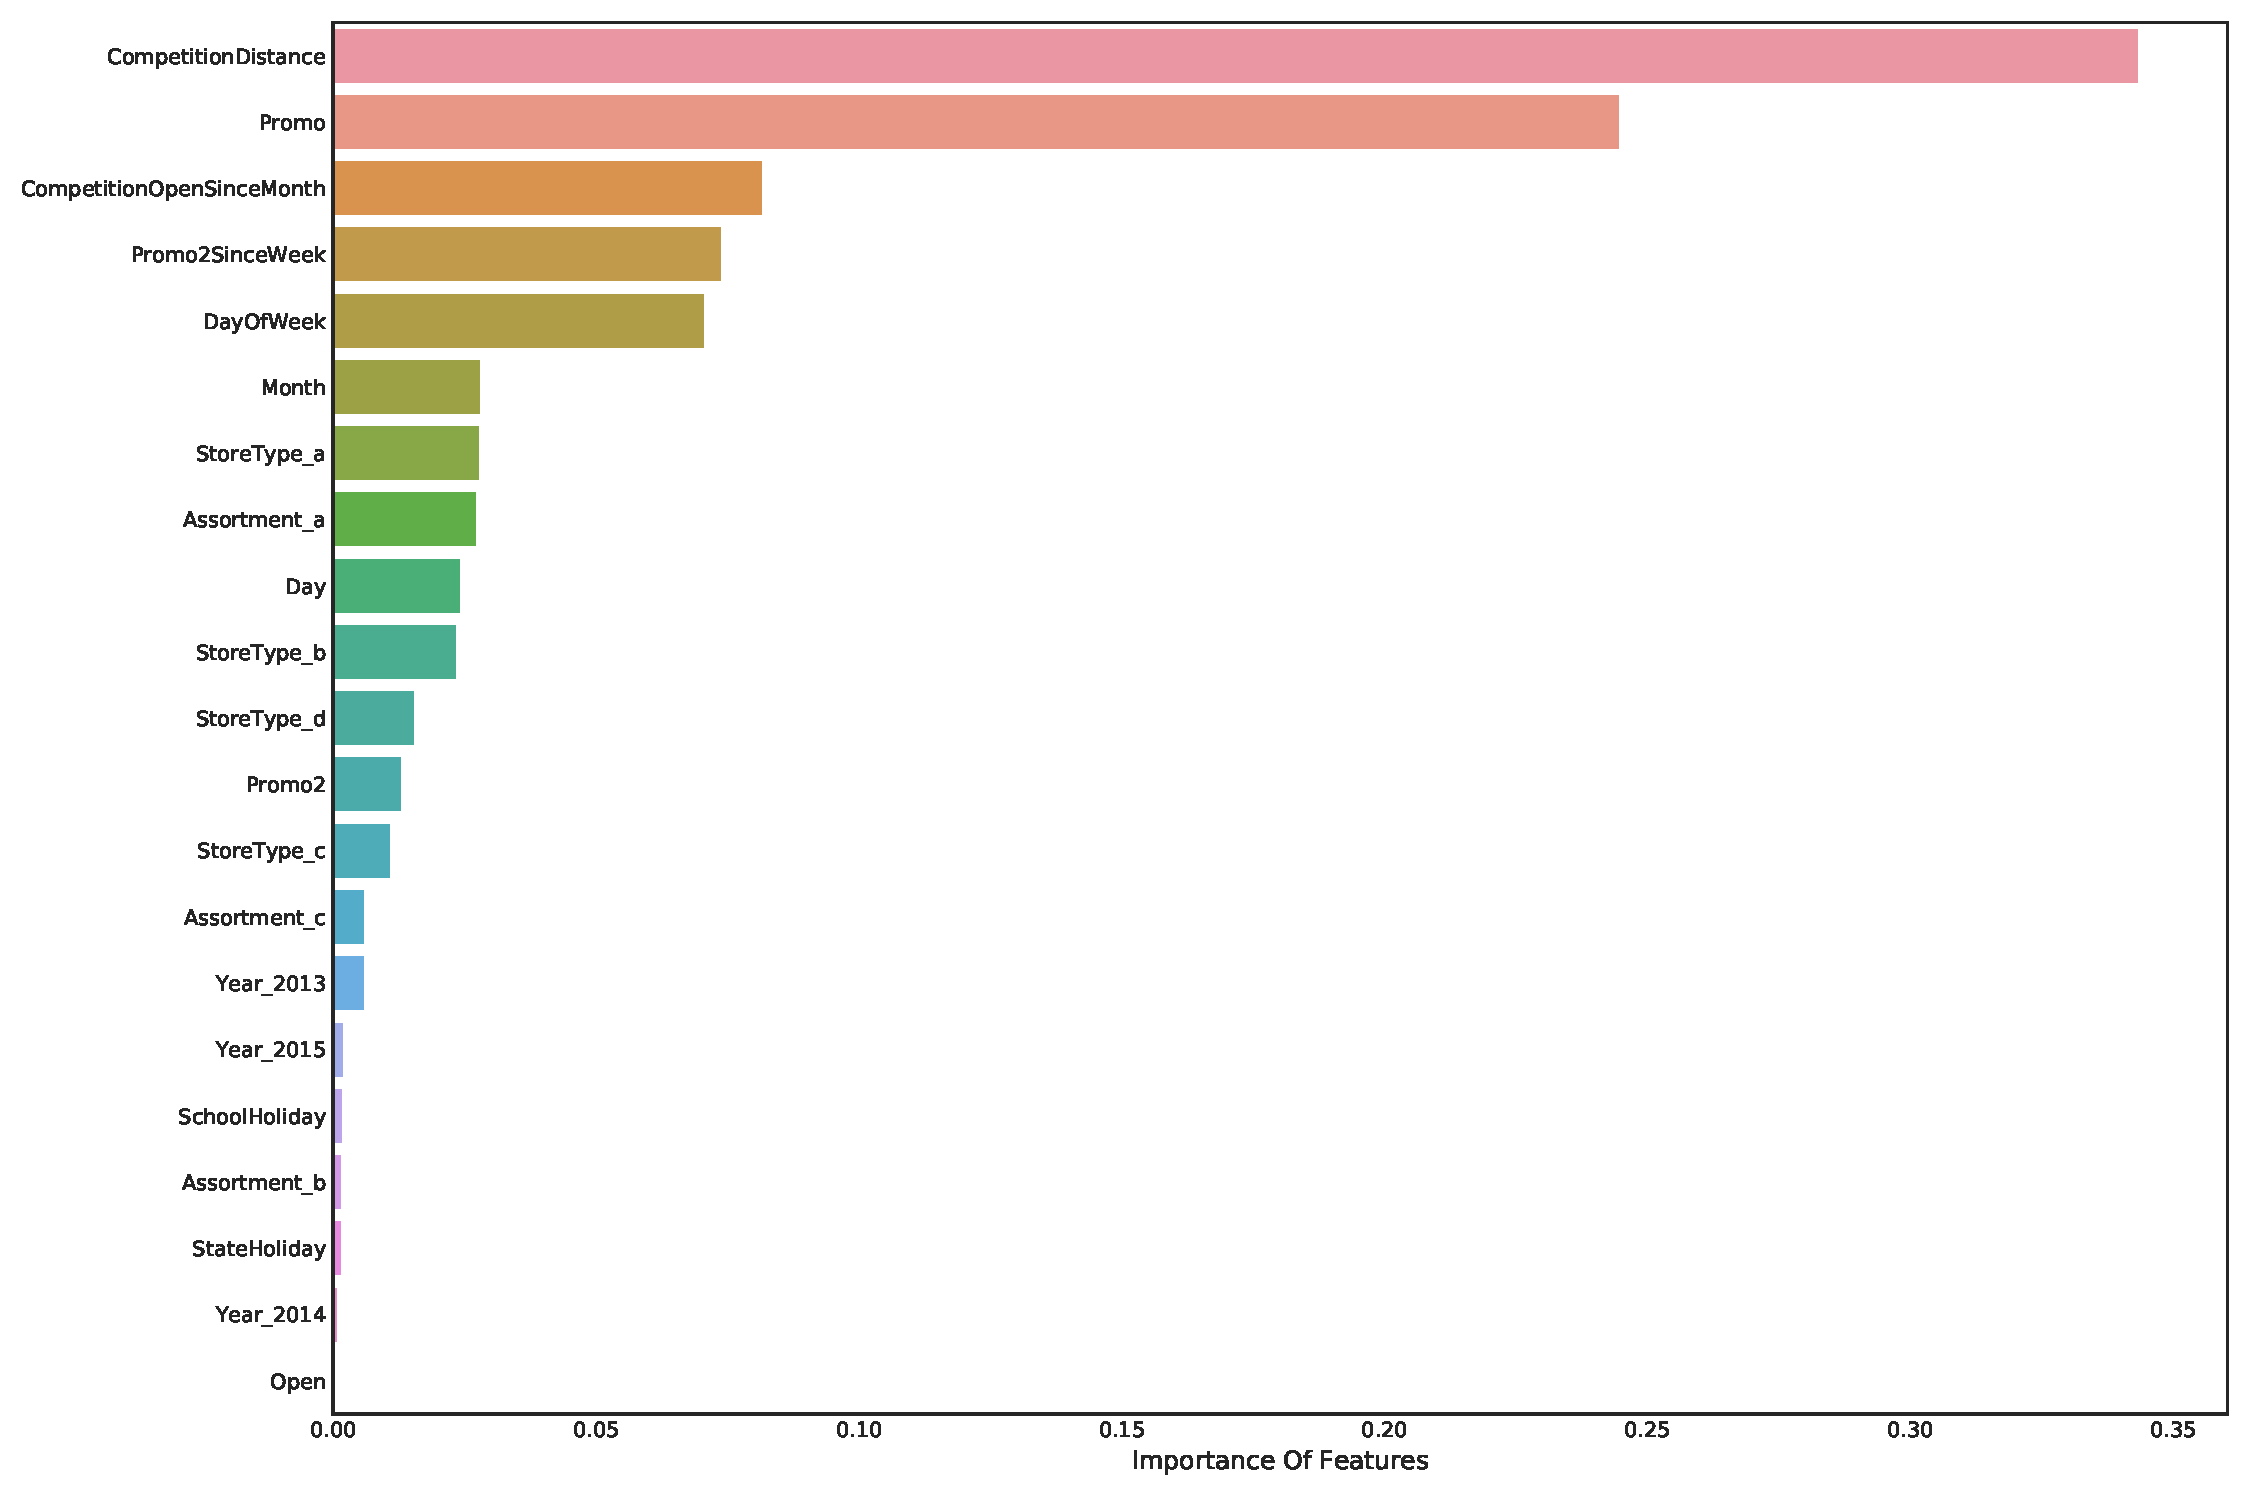
\includegraphics[width=0.9\columnwidth]{formulas/importance_of_features.pdf}
\caption{Importance Of Features caculated by RandomForest}
\label{fig:Importance Of Features}
\end{figure}

'StateHoliday' and 'SchoolHoliday' are insignificant in RandomForestClassifier, however, 'StateHoliday' in Heatmap have certain level of correlation with 'Sales'. I prefer dropping 'SchoolHoliday' alone rather than removing both of the columns.

Heatmap and RandomForestClassifier provide adequate reason for data cleaning. Moreover,due to the fluctuation of seasonal sales shown in Figure 2, using log-transformed sales could make this dependent variable looks more linear by narrowing the fluctuated sales gap.

\section{Modeling Method}
Train dataset was splitted into training dataset and validation dataset, while test dataset stay unchanged \cite{shah2017train}.

\begin{itemize}
    \item \textit{Training Dataset} -- The sample of data used to fit the model.
    \item \textit{Validation Dataset} -- The sample of data used to provide an unbiased evaluation of a model fit on the training dataset while tuning model hyperparameters.
    \item \textit{Test Dataset} -- The sample of data used to provide an unbiased evaluation of a final model fit.
\end{itemize}

Linear models as well as tree-based methods are employed in setting up the model.  Root Mean Square Error (RMSE) is the benchmark to measure model accuracy.

\subsection{Linear Models}
\subsubsection{Ordinary Least Squares (OLS)}
Ordinary Least Squares (OLS) is the most common estimation method for linear models \cite{fox1997applied}.
\begin{equation}
y_i=\beta_1x_{i2}+\beta_2x_{i2}+\dots+\beta_nx_{in}+\varepsilon_i
\end{equation}

in vector form
\begin{equation}
y_i=x_i^T\beta+\varepsilon_i
\end{equation}

can also be written in matrix form
\begin{equation}
y=X\beta+\varepsilon
\end{equation}

The overall moedel fit is measured by Sum of Squared Residuals (SSR):
\begin{equation}
 S(b)=\sum_{i=1}^{n}(y_i-x_i^Tb)^2=(y-Xb)^T(y-Xb)
\end{equation}

The value of $b$ which minimizes this sum is called the OLS estimator for $\beta$
\begin{equation}
\hat{\beta}=\operatorname*{argmin}_b S(b)=(X^TX)^{-1}X^Ty
\end{equation}

Root mean squared error is the square root of the sum of squared residuals divided by the number of degrees of freedom.

\subsubsection{Ridge Regression}
In Ridge Regression, the loss function is augmented in such a way that not only minimize the sum of squared residuals but also penalize the size of parameter estimates \cite{jain2016complete}, in order to shrink them towards zero:
\begin{equation}
L_{ridge}=\sum_{i=1}^{n}(y_i-x_i^T\hat{\beta})^2+\lambda\sum_{j=1}^{m}\hat{\beta}_j^2=\|y-X\hat{\beta}\|_2^2+\lambda\|\hat{\beta}\|_2^2
\end{equation}
where $\|\cdot \|_2$ is the Euclidean norm.
\begin{equation}
\hat{\beta}_ridge=(X^TX+\lambda I)^{-1}X^Ty
\end{equation}
where $I$ denotes the identity matrix, the parameter $\lambda$ is the regularization penalty. As $\lambda$ $\to$ $0$ , $\hat{\beta}_{ridge}$ $\to$  $\hat{\beta}_{OLS}$ ; as $\lambda$ $\to$ $\infty$ , $\hat{\beta}_{ridge}$ $\to$ $0$.

\subsubsection{Lasso Regression}
Lasso (least absolute shrinkage and selection operator) is a regression analysis method that performs both variable selection and regularization \cite{tibshirani1996regression}. Mathematics behind lasso regression is quiet similar to that of ridge, only difference is that instead of penalizing sum of squared coefficients($\ell_2$ penalty), lasso penalizes the sum of their absolute values($\ell_1$ penalty). Lasso loss functions is defined as:
\begin{equation}
L_{lasso}=\sum_{i=1}^{n}(y_i-x_i^T\hat{\beta})^2+\lambda\sum_{j=1}^{m}|\hat{\beta}_j|=\|y-X\hat{\beta}\|_2^2+\lambda\|\hat{\beta}\|_1
\end{equation}

\subsection{Tree-Based Models}
\subsubsection{Decision Tree}
A decision tree is a flowchart-like tree structure where an internal node represents feature, the branch represents a decision rule, and each leaf node represents the outcome.Since it often mimics the human level thinking, decision tree is one of the easiest and popular classification algorithms to understand the data and make some good interpretations \cite{freund1999alternating}.

There are couple of algorithms there to build a decision tree, in this paper, I choose the algorithms that are referred to as CART or Classification and Regression Trees.

Recursive Binary Splitting is a common used technique for deciding on which features to choose and what conditions to use for splitting, along with knowing when to stop. The greedy algorithm, which makes the root node as best predictor/classifier via a function that calculates how much accuracy each split will cost, choose the split that costs least.

Let the data at node $m$ be represented by $Q$. For each candidate split $\theta =(j,t_m)$ consisting of a feature $j$ and threshold $t_m$, partition the data into $Q_{left}(\theta)$ and $Q_{right}(\theta)$ subsets
\begin{equation}
Q_{left}(\theta)=(x,y)|x_j\leq t_m
\end{equation}
\begin{equation}
Q_{right}(\theta)=Q\setminus Q_{left}(\theta)
\end{equation}
The impurity at $m$ is computed using an impurity function $H()$
\begin{equation}
G(Q,\theta)=\frac{n_{left}}{N_m}H(Q_{left}(\theta))+\frac{n_{right}}{N_m}H(Q_{right}(\theta))
\end{equation}
Select the parameters that minimises the impurity
\begin{equation}
\theta_\ast=\operatorname*{argmin}_\theta G(Q,\theta)
\end{equation}
Recurse for subsets $Q_{left}(\theta_\ast)$ and $Q_{right}(\theta_\ast)$ until the maximum allowable depth is reached, $N_m<min_{samples}$ or $N_m=1$.

\subsubsection{Random Forest}
Decision trees are a popular method for various machine learning tasks. Nevertheless, deep-growing trees may tend to learn highly irregular patterns that lead to overfitting. Random forests are a way of averaging multiple deep decision trees, trained on different parts of the same training set, with the goal of reducing the variance.

Like you can already see from it’s name, random forest creates a forest and makes it somehow random. As shown in Fig \ref{fig:Random Forest}
\begin{figure}[ht]
\centering
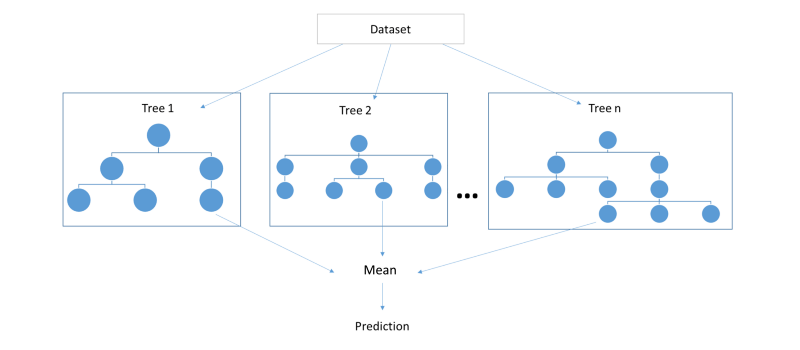
\includegraphics[width=0.9\columnwidth]{formulas/randomforest.png}
\caption{Random forest builds multiple decision trees and merges them together to get a more accurate and stable prediction. from \cite{Vaibhav:2018:Online}}
\label{fig:Random Forest}
\end{figure}
, the "forest" is an ensemble of decision trees, most of the time trained with the bagging method whose general idea is: a combination of learning models increases the overall result. Besides, random forest can be used for both classification and regression tasks, acquire a great result even without hyper-parameter tuning most of the time.

Random Forest adds additional randomness to the model, while growing the trees. Instead of searching for the most important feature while splitting a node, it searches for the best feature among a random subset of features. This results in a wide diversity that generally results in a better model.Therefore, in Random Forest, only a random subset of the features is taken into consideration by the algorithm for splitting a node.

\subsubsection{Gradient Boosting}
As well as random forest, gradient boosting in another popular ensemble methods. Gradient boosting and random forest differ in the way the trees are built: the order and the way the results are combined \cite{ogutu2011comparison}.

\hspace*{6mm}\textit{Input:}

\hspace*{6mm}\texttt{training set $\{(x_{i},y_{i})\}_{i=1}^{n}$, a differentiable loss function $L(y,F(x))$,\\\hspace*{10mm} number of iterations $M$.}

\hspace*{6mm}\textit{Algorithm:}

\hspace*{6mm}\texttt{1. Initialize model with a constant value:}
\begin{equation}
F_0(x)=\operatorname*{argmin}_\gamma\sum_{i=1}^{n}L(y_i,\gamma)
\end{equation}

\hspace*{6mm}\texttt{2. For $m=1$ to $M$:}\\
\hspace*{20mm}\texttt{1) Compute so-called pseudo-residuals:}
\begin{equation}
r_{im}=-[\frac{\partial L(y_i,F(x_i)}{\partial F(x_i)}]_{F(x)=F_{m-1}(x)} \hspace*{10mm}for\hspace{2mm} i=1,\dots,n
\end{equation}

\hspace*{20mm}\texttt{2) Fit a base learner (e.g.tree) $h_{m}(x)$ to pseudo-residuals, \\ \hspace*{34mm}i.e.train it using the training set ${(x_{i},r_{im})}_{i=1}^{n}$.}

\hspace*{20mm}\texttt{3) Compute multiplier $\gamma _{m}$ by solving the following one-dimensional\\\hspace*{34mm}optimization problem:}
\begin{equation}
\gamma_m=\operatorname*{argmin}_\gamma\sum_{i=1}^{n}L(y_i,F_{m-1}(x_i)+\gamma h_m(x_i))
\end{equation}

\hspace*{20mm}\texttt{4) Update the model:}
\begin{equation}
F_m(x)=F_{m-1}(x)+\gamma_mh_m(x)
\end{equation}

\hspace*{6mm}\texttt{3. Output $F_{M}(x)$.}

Boosting is a method of converting weak learners into strong learners. In boosting, each new tree is a fit on a modified version of the original data set. Gradient boosting build trees one at a time, where each new tree helps to correct errors made by previously trained tree, see Fig \ref{fig:Boosted Trees}
\begin{figure}[ht]
\centering
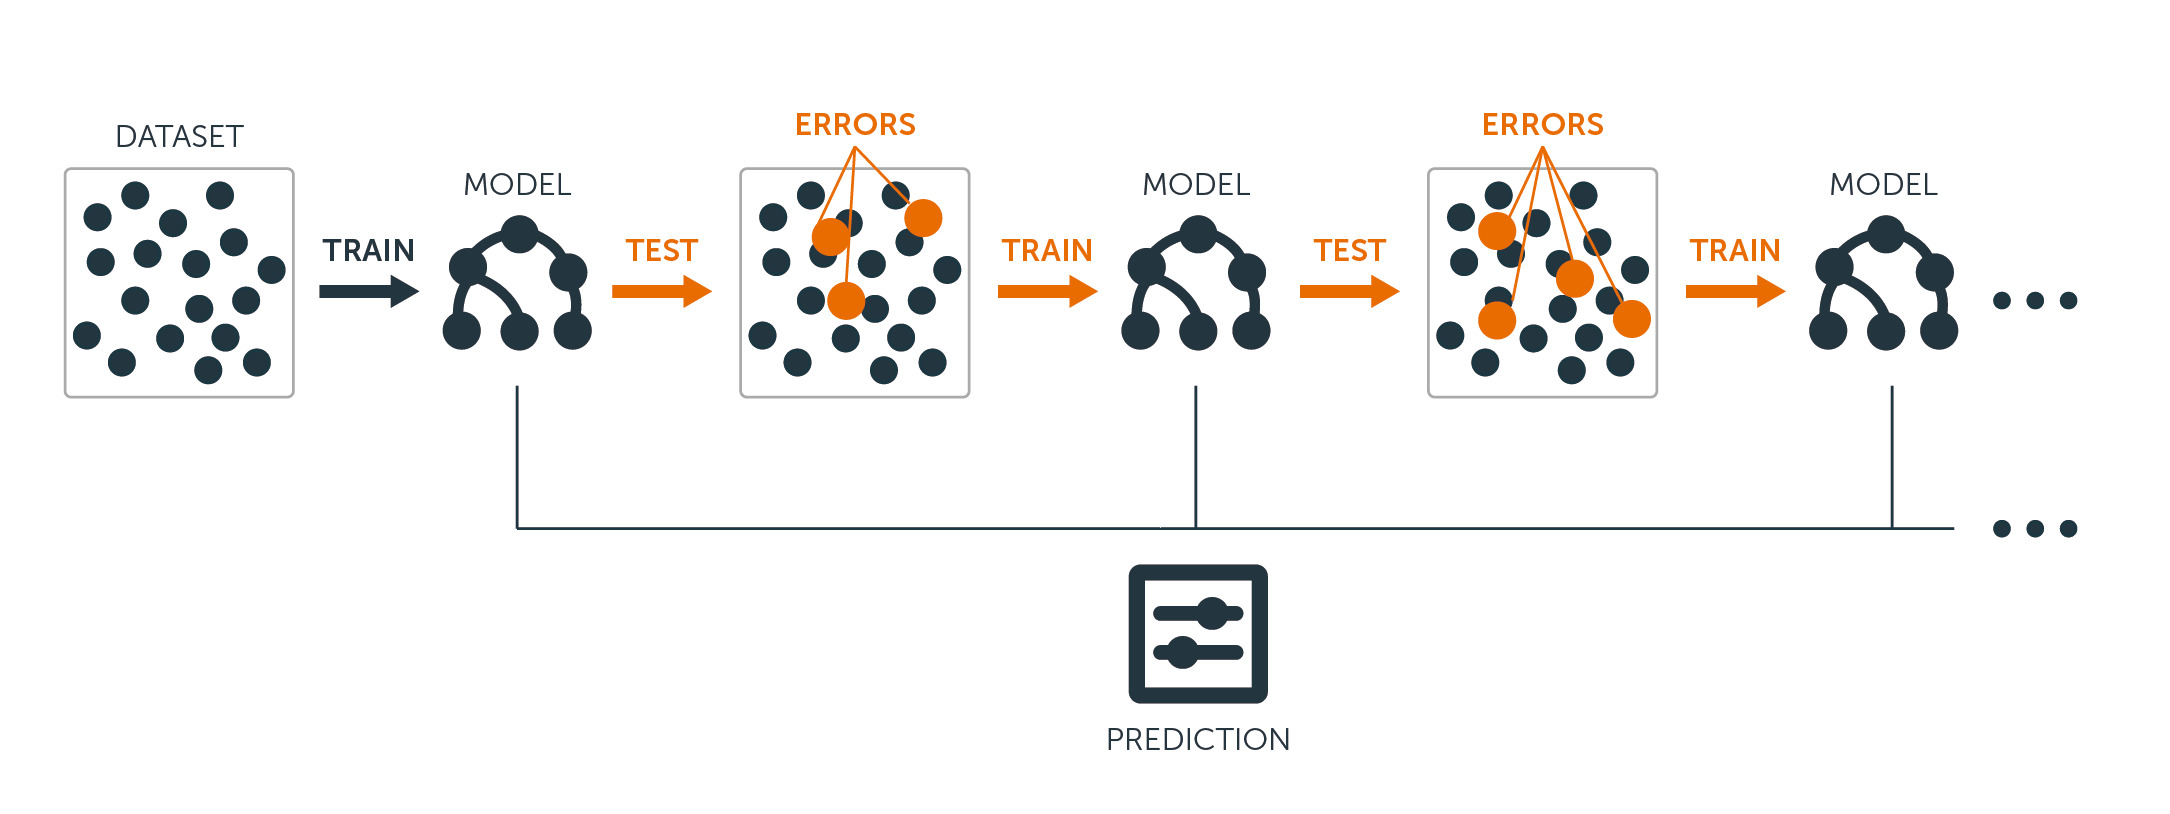
\includegraphics[width=0.9\columnwidth]{formulas/boosted-trees-process.png}
\caption{Iterative modeling processes improve the prediction function results. from \cite{Diogo:2018:Online}}
\label{fig:Boosted Trees}
\end{figure}
It has been shown that gradient boosting performs better than random forest if parameters tuned carefully.

\section{Experiment and Results}
All the regressions and classifications were  executed via scikit-learn, which is a machine learning library for Python. Cross-validation, an important techniques for assessing how the results of a model will generalize to an independent data set, was used to examine the efficiency of the models. I set $cv=5$, which means 5-fold cross-validation. Fig \ref{fig:k-fold cross-validation}
\begin{figure}[ht]
\centering
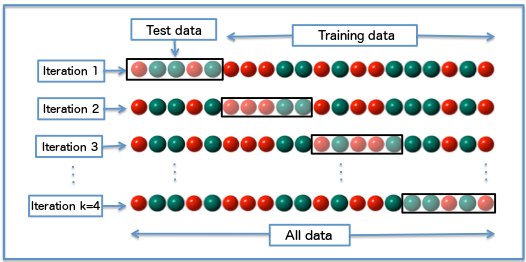
\includegraphics[width=0.7\columnwidth]{formulas/K-fold_cross_validation.jpg}
\caption{k-fold cross-validation with k=4. from \cite{Fabian:2016:Online}}
\label{fig:k-fold cross-validation}
\end{figure}
explains how k-fold cross-validation works.

Fig \ref{fig:rmse}
\begin{figure}[ht]
\centering
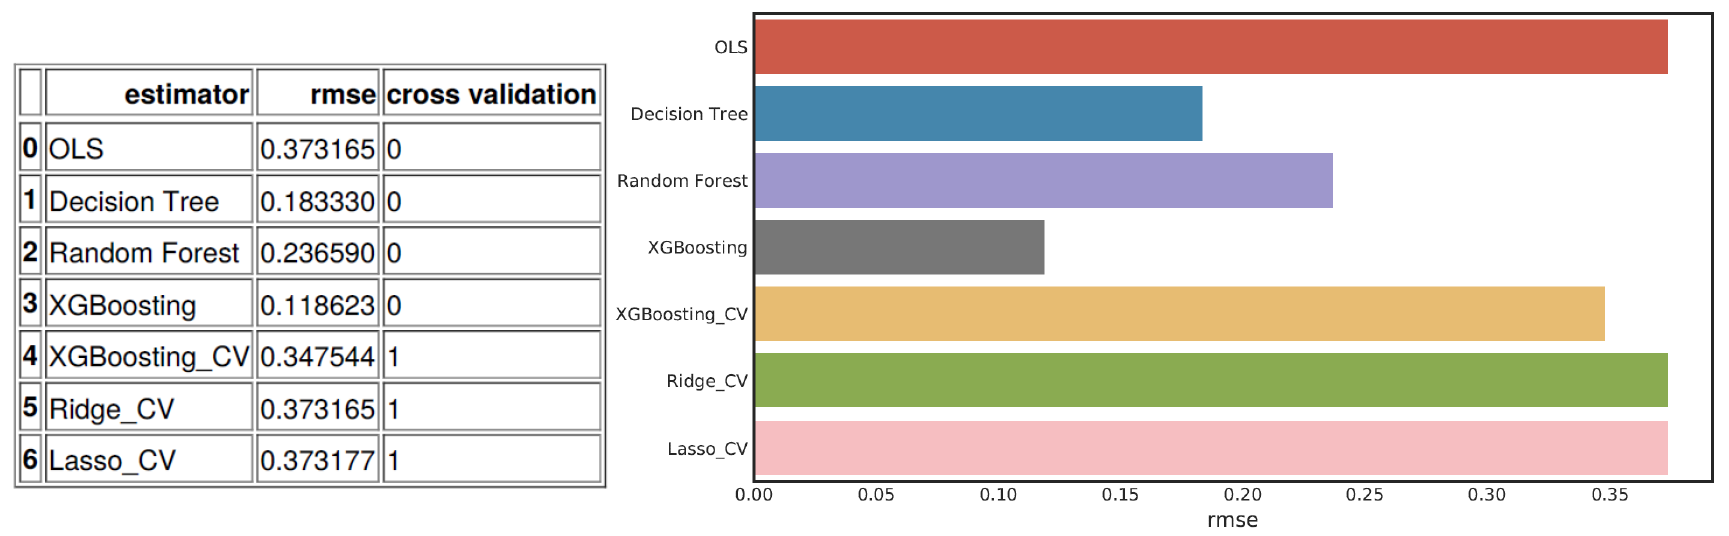
\includegraphics[width=0.9\columnwidth]{formulas/rmse.png}
\caption{comparison between model RMSEs}
\label{fig:rmse}
\end{figure}
demonstrates scores for each model, where cross validation column with label 1 represents 5-fold cross-validation was used in model construction.

The performance of XGBoosting regressor is the best of all non-cross-validated model. Afterwards, I run an extra cross-validated version of it to verify whether it would be the tops among the whole cross-validated models. As a result, rmse of XGBoosting is 6.87\% lower than Ridge regressor.

After applying this cross-validated XGBoosting estimator to the test dataset to generate my final prediction, I uploaded this final result to Kaggle.
\begin{figure}[h]
\centering
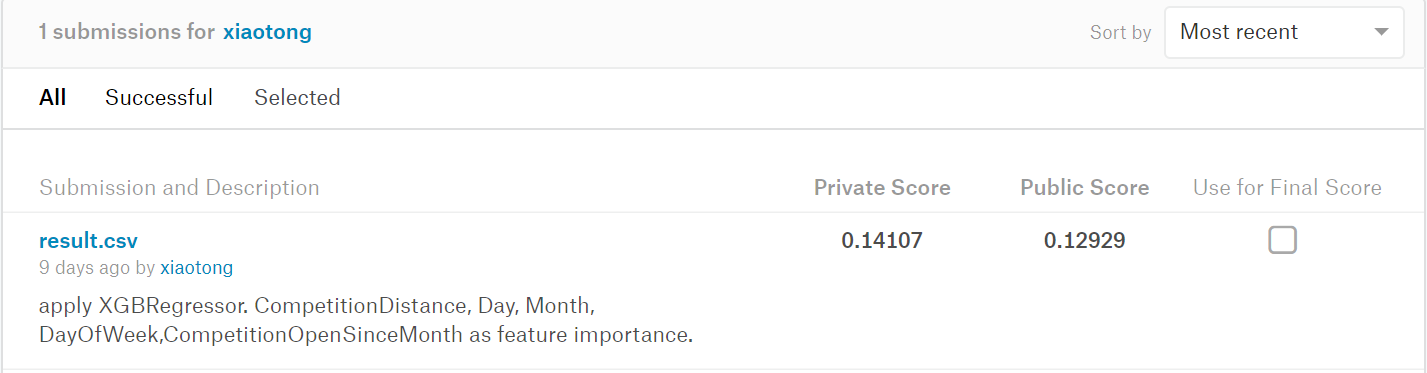
\includegraphics[width=0.7\textwidth]{formulas/submission.png}
\end{figure}

Although the score are quite low, it's still a good beginning for further improvement. The picture bellow shows the public  leaderboard of the Kaggle competition.

\begin{figure}[h]
\centering
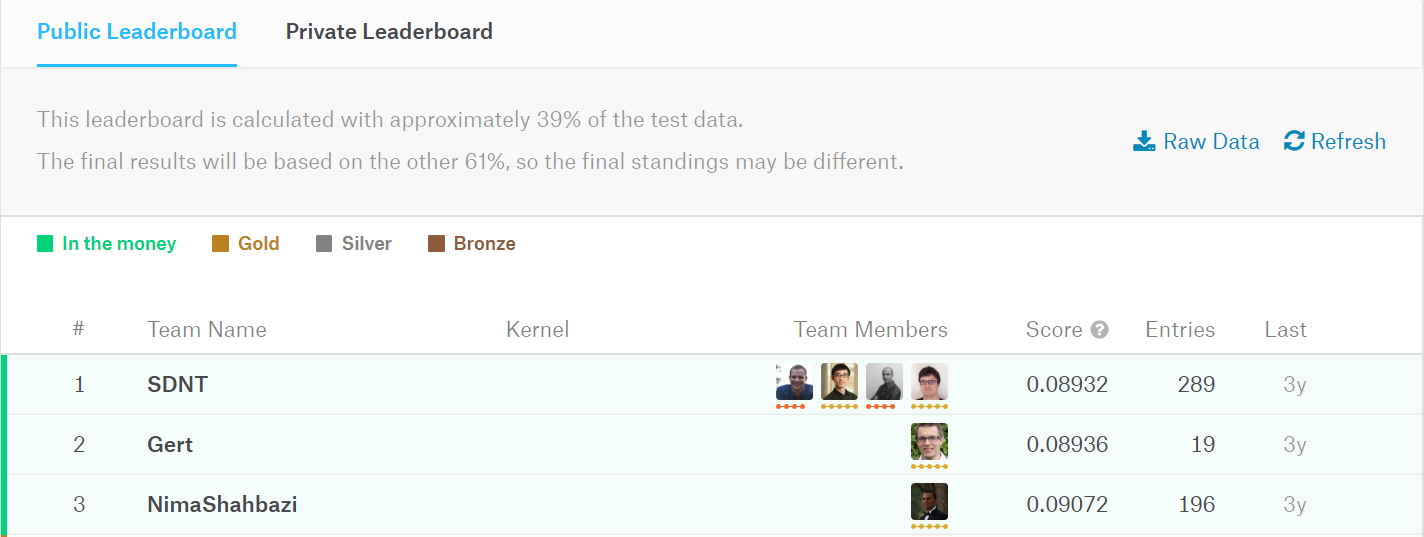
\includegraphics[width=0.7\textwidth]{formulas/leader.png}
\end{figure}

\section{Conclusion and Future work}

In practice, data cleaning and regression model choosing is not so difficult. Packages like pandas, numpy and scikit-learn are able to deal with most of the relative problems. whereas, feature selection is the top priority, since a good subset of variables can increase the accuracy of trained model and avoid overfitting in the meanwhile. The way I convert categorical data into numerical data is the most tricky part among the rest during feature extraction.

Gradient boosting is a great algorithm for model building \cite{chen2015xgboost}. It prevails over the other estimators with obvious advantage \cite{ke2017lightgbm}. There are lots of evidence based on the Kaggle competitions shows that XGBoosting is a silver bullet for competition participants.

Time series analysis and forecasting would be an alternative method to predict Rossmann store sales. The historical data in train dataset is a series of data points indexed in time order. In addition, a seasonal dependency could be easily discoverd according to Fig 2. The only fly in the ointment is that the time period in the historical data is just 2.5 years, which is too short to investigate secular trend. Above all, I could theoretically identify patterns such as seasonal variations, cyclical fluctuations, irregular variations in time series data \cite{han1999efficient}. ARIMA(Autoregressive Integrated Moving Average) models, grid search and validating forecasts might be applied in the further improvement.


\bibliography{refs}



% \appendix

% The chngctr package is needed for the following lines.
% \counterwithin{table}{section}
% \counterwithin{figure}{section}

\end{document}
